\documentclass[a4paper,11pt]{article}
\usepackage{commonpackages}

\begin{document}
\title{CSS}
\date{}
\maketitle

\section{Théorie}
Le langage \textbf{CSS} (Cascading Style Sheet en français feuilles de style en cascade) permet de mettre en forme les documents HTML. Il permet notamment de modifier la police, la couleur, la taille et l'emplacement du contenu.\\
CSS est un langage basé sur des règles: il permet de définir des règles de style pour un type d'élément donné, par exemple les titres principaux <h1></h1> ou les paragraphes <p></p>

\subsection{Structure du code CSS}
\begin{tabular}{l l}
sélecteur \{ & La règle commence par un sélecteur\\
\quad propriété1: valeur1;  & à chaque propriété correspond une valeur est attribuée\\
\quad propriété2: valeur2; & \\
\}& \\
\end{tabular}

\begin{tabular}{ll}
\begin{minipage}{1\textwidth}
\begin{code}{css}
h1 {
  color: green;
  text-align: center;
}
\end{code}
\end{minipage}&
\begin{minipage}{1\textwidth}
Défini le style du titre principal\\
La couleur du texte est verte\\
L'alignement du texte est centré\\
\end{minipage}\tabularnewline
\end{tabular}\par

\begin{tabular}{cc}
\begin{minipage}{1\textwidth}
\begin{code}{css}
p {
  font-family: verdana;
  font-size: 20px;
}
\end{code}
\end{minipage}&
\begin{minipage}{1\textwidth}
Défini le style des paragraphes\\
La police utilisée est verdana\\
La taille de la police est 20 pixels\\
\end{minipage}\tabularnewline
\end{tabular}\par


\subsection{Référencement - Balise <link \dots>}
Comme le ficher HTML (.html) et le fichier CSS (.css) sont deux fichiers distincts, il faut ajouter au document HTML une référence au fichier CSS. Cela se fait dans le <head> du document HTML avec la balise <link>.
La balise <link> a deux attributs: rel (précise à quoi sert le fichier référencé) et href (chemin d'accès au document):
\begin{code}{html}
<link href="style.css" rel="stylesheet" type="text/css" />
\end{code}

\subsection{Sélecteurs}
Dans ce cours, nous allons travailler sur 3 types de sélecteurs:
\begin{itemize}
\item sélecteur de type
\item sélecteur d'identifiant
\item sélecteur de classe
\end{itemize}

\subsubsection{Sélecteur de type}
Le sélecteur de type permet d'appliquer un style à toutes les balises de même type (h1, h2, p, \dots).
Il est de la forme: \par
\begin{code}{css}
h1 {
  color: green;
  text-align: center;
}
\end{code}\par
Ce style s'appliquera au contenu de toutes les balises <h1>…</h1>

\subsubsection{Sélecteur d'identifiant}
Le sélecteur d'identifiant permet d'appliquer un style à un élément précis. Pour cela, il faut ajouter un nouvel attribut id à la balise HTML concernée.\par

\begin{tabular}{|c|c|}
\hline
\centering Fichier HTML & Fichier CSS\tabularnewline
\hline
\begin{minipage}{1\textwidth}
\begin{code}{html}
<p id = "intro">
  Dans ce paragraphe ...
</p>
\end{code}
\end{minipage}&
\begin{minipage}{1\textwidth}
\begin{code}{css}
#intro{
  text-align: justify;
  color: green;
}
\end{code}
\end{minipage}\tabularnewline
\hline
\end{tabular}\par
Ce style s'appliquera qu'à la balise dont l'id est "intro".

\subsubsection{Sélecteur par classe}
Le sélecteur de classe permet d'appliquer un style à plusieurs éléments qui appartiennent à un même classe (groupe). Pour cela, il faut ajouter un nouvel attribut class à la balise HTML concernée.\par

\begin{tabular}{|c|c|}
\hline
\centering Fichier HTML & Fichier CSS\tabularnewline
\hline
\begin{minipage}{1\textwidth}
\begin{code}{html}
<p class = "centre">
  Dans ce paragraphe ...
</p>
\end{code}
\end{minipage}&
\begin{minipage}{1\textwidth}
\begin{code}{css}
.centre{
  text-align: center;
}
\end{code}
\end{minipage}\tabularnewline
\hline
\end{tabular}\par
Ce style s'appliquera qu'aux balises dont la classe est "centre".

Tuto: \href{https://developer.mozilla.org/fr/docs/Learn/Getting_started_with_the_web/CSS_basics}{MND - CSS}


\subsection{Conteneurs <div>}
\begin{multicols}{2}
\begin{minipage}{1\textwidth}
Un conteneur est un élément qui contient plusieurs éléments et qui est défini comme un bloc.
Il est défini en HTML par la balise <div> \dots </div>. Dans le fichier CSS, il est possible de définir différentes propriétés d'un bloc, comme la hauteur (height), la largeur (width), la marge intérieure (padding), la marge extérieure (margin) ou la bordure (border).
\end{minipage}
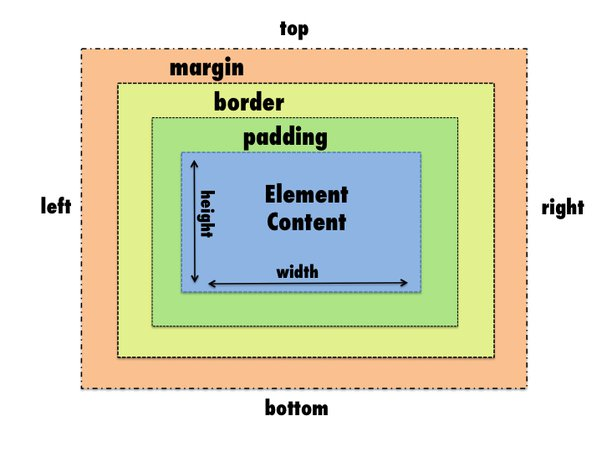
\includegraphics[width= 1\textwidth]{images/conteneur.png}
\end{multicols}

\begin{tabular}{|c|c|}
\hline
\centering Fichier HTML & Fichier CSS\tabularnewline
\hline
\begin{minipage}{1\textwidth}
\begin{code}{html}
<div id="mon_conteneur">
  <h2>Mon sous-titre<h2/>
  <p> Lorem ipsum dolo sit amet.</p>
</div>
\end{code}
\end{minipage}&
\begin{minipage}{1\textwidth}
\begin{code}{css}
#mon_conteneur{
  background-color: red;
  width: 100%;
  height: 400px;
  border: 2px solid;
  padding: 1em;
}
\end{code}
\end{minipage}\tabularnewline
\hline
\end{tabular}\par

Tuto: \href{https://developer.mozilla.org/fr/docs/Web/HTML/Element/div}{MDN - div}

\section{Exercices}
\subsection{Exercice}
But: Appliquer un fichier CSS au document index.html.
\begin{enumerate}
\item Sur Moodle, télécharger le document \textbf{style.css}.
\item Sauvegarder ce document sur OneDrive dans le dossier informatique.
\item Sur replit.com, il faut remplacer le fichier style.css par celui que vous venez de télécharger:
\begin{enumerate}
  \item Effacer le fichier \textbf{style.css} déjà présent.
  \item Télécharger votre fichier en cliquant sur les 3 points verticaux et en séléctionnant \textbf{Upload file}. Choisir le fichier \textbf{ style.css} que vous avez sauvergarder sur votre OneDrive.
\end{enumerate}
\item Ajouter le référencement à la page \textbf{style.css} dans le <head> du document \textbf{index.html}. (cf. 4.2)
\item Appuyer sur le bouton \textbf{Run}.
\end{enumerate}

\subsection{Exercice}
\begin{enumerate}
\item Qu'est-ce qui a changé?
\item Cliquer sur \textbf{style.css} pour que le document s'afficher et essayer de le comprendre.
\begin{enumerate}
  \item À quels éléments s'appliquent les différentes propriétés?
  \item Quelle est la différence entre h1{\dots} et \#source{\dots}? Quand va-t-on utiliser le deuxième?
\end{enumerate}
\item Vous allez maintenant modifier cette page (pour valider une modification, appuyer sur \textbf{Run}):
\begin{enumerate}
  \item Modifier la couleur des titres et des sous-titres. Vous pouvez utiliser les noms en anglais ou le code RGB.\\
  \href{https://www.rapidtables.com/web/color/RGB_Color.html}{Liste des couleurs}
  \item Modifier la police de caractère (font) des titres (pas des sous-titres) en  "fantasy".
  \item Modifier la couleur de fond de la page HTML.
  \item Ajouter une couleur de fond aux titres et aux sous-titres.
  \item Modifier le code pour que toutes les sources s'affichent en gris foncé. (Il faut utiliser un sélecteur de classe.)
  \item Ajouter une bordure au tableau.
\end{enumerate}
\end{enumerate}

\subsection{Exercice}
À vous de jouer. Réfléchir à la structure de votre site internet:
\begin{enumerate}
\item Quelles seront les différentes pages?\\
Sur replit.com, il est nécessaire que la première page de votre site s'appelle \textbf{index.html}. Vous pouvez en créer d'autres et les référencer avec des liens pour pouvoir naviguer entre les différentes pages de votre site.
\item Quel sera le style de votre site? Pouvez-vous le réaliser avec les outils vus en classe? Sinon rechercher sur internet comment faire.
\end{enumerate}

\section{Liens pour des tutos}
\href{https://developer.mozilla.org/fr/docs/Web/HTML}{Tuto pour HTML}
\href{https://developer.mozilla.org/fr/docs/Web/CSS}{Tuto pour CSS}
\href{https://www.w3schools.com/ }{Tuto en anglais}

\end{document}
